\documentclass[10pt]{article}\usepackage[margin=.65in]{geometry}\usepackage[T1]{fontenc}\usepackage{graphicx}\setlength{\parindent}{0pt}\setlength{\parskip}{7pt}\sloppy\begin{document}{\large Two word finds compose with a distinct-root union}\par Four new declarations compiled, together with seven adapted dependency declarations and six fixed controls. Seventeen separate named axiom readbacks passed. Independent source-fidelity review is pending.\par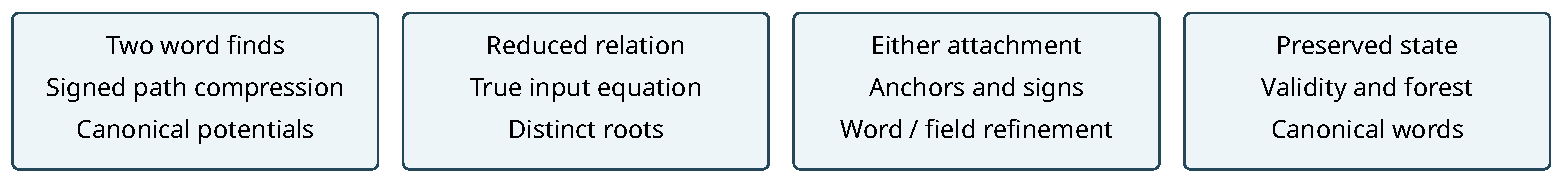
\includegraphics[width=\linewidth]{diagram.pdf}\par Integration correction. The existing word-find and word-union modules could not be imported together: both declared SignedWord.pairDecode for different types. The original failed import is retained. Three isolated union-module copies now name the anchor-pair decoder anchorPairDecode and redirect their imports. Exact transformation checks establish that the copied proof bodies have no other textual change. Original producer packets remain unchanged; the combined imports now pass.

Construction. reducedUnionPot\_correct connects canonical machine-word reduced labels to the existing field potential. branchWord\_refines and branchWord\_good handle both attachment directions. distinct\_union\_after\_two\_word\_finds composes two source-modeled Run relations, the true incoming relation, and a distinct-root union. Its conclusion preserves canonical graph coefficients and fixed anchors, decoded relation validity, and existence of a forest rank, permitting subsequent root searches under the existing termination theorem.

Assumptions. The modulus is prime, positive and at most 2\textasciicircum{}63. Inputs have canonical coefficients and signed labels in {1,-1}; the initial graph is a forest with a valid value assignment and fixed anchors. The incoming equation is an explicit premise. Its geometric truth must be supplied by the relation producer. The two roots are distinct. The result models either attachment orientation; it does not yet establish the native size-vector updates, size-based choice, array growth or complete collector execution.

Controls. A three-vertex fixture follows a nontrivial signed path and then finds a distinct root. The reduced union label is checked exactly. Forward attachment transfers an anchor to the new parent; backward attachment preserves the existing parent anchor. A zero sign is rejected. These are bounded proof controls, not a new scientific cohort or timing sample.

Retained attempts. The packet preserves the original import collision, failed proof-development attempts and a prematurely attempted control import before its dependency compiled. The final main/control/readback receipts have exit zero with unchanged bound inputs; the false theorem has exit one. Imported compiled dependencies were reused, not independently rebuilt. Before/after hashes do not prove absence of transient edits. The audit checks all seventeen names and permits only propext, Classical.choice and Quot.sound, with empty, wrong-name and sorryAx rejection controls.

Next review. Publish immutable adapted sources and receipts, then obtain independent review of native union orientation, signed offsets, anchor behavior, overflow bounds and the two-find composition. Keep native size accounting and producer-edge truth as explicit remaining obligations. This graph records proof dependencies; no scientific execution or measured cost changed. The original cohort and campaign limits remain unchanged.
\end{document}